% !TeX program = lualatex
% !TeX encoding = UTF-8
% !TeX spellcheck = fr_FR

\documentclass[12pt,a4paper,openany]{report}

% ==============================================================================
% 1. MOTEUR & LANGUE (Spécifique LuaLaTeX)
% ==============================================================================
\usepackage{fontspec}
\usepackage{polyglossia}
\setmainlanguage{french}
\setotherlanguage{english}

% ==============================================================================
% 2. MISE EN PAGE & STRUCTURE
% ==============================================================================
\usepackage{geometry}
\geometry{left=2.5cm, right=2.5cm, top=3cm, bottom=3cm, headheight=30pt}

\usepackage{fancyhdr}
\usepackage{titlesec}
\usepackage{tocloft}
\usepackage{titletoc}

% ==============================================================================
% 3. TYPOGRAPHIE & TEXTE
% ==============================================================================
\usepackage{setspace}
\usepackage{xcolor}
\usepackage{csquotes}
\usepackage{enumitem}
\usepackage{indentfirst}
\usepackage{hyphenat}
\usepackage[skins]{tcolorbox}
% ==============================================================================
% 4. MATHÉMATIQUES & SYMBOLES
% ==============================================================================
\usepackage{amsmath}
\usepackage{amssymb}
\usepackage{amsfonts}
\usepackage{mathtools}
\usepackage{bm}


% ==============================================================================
% 5. GRAPHISMES & DIAGRAMMES
% ==============================================================================
\usepackage{graphicx}
\usepackage{tikz}
\usetikzlibrary{positioning, shapes.geometric, arrows.meta, calc}
\usepackage{pgfplots}
\pgfplotsset{compat=1.18}
\usepackage{caption}
\usepackage{subcaption}
\usepackage{float}

% ==============================================================================
% 6. TABLEAUX
% ==============================================================================
\usepackage{booktabs}
\usepackage{longtable}
\usepackage{array}
\usepackage{multirow}
\usepackage{tabularx}
\usepackage{colortbl}

% ==============================================================================
% 7. CODE SOURCE & LISTINGS
% ==============================================================================
\usepackage{listings}
\usepackage{lstautogobble}

% ==============================================================================
% 8. LIENS & RÉFÉRENCES
% ==============================================================================
\usepackage{hyperref}
\usepackage{bookmark}
\usepackage{url}
\usepackage{hypcap}

% ==============================================================================
% 9. UTILITAIRES DIVERS
% ==============================================================================
\usepackage{pdfpages}
\usepackage{imakeidx}
\usepackage{lastpage}
\usepackage{lipsum}

% ==============================================================================
% POLICES ET TYPOGRAPHIE
% ==============================================================================
\setmainfont{Latin Modern Roman}
\setsansfont{Latin Modern Sans}
\setmonofont{Latin Modern Mono}

% ==============================================================================
% COULEURS ET STYLE (Palette Professionnelle)
% ==============================================================================
\definecolor{primary}{RGB}{0,51,102}       % Bleu Nuit Profond
\definecolor{secondary}{RGB}{0,102,204}    % Bleu Plus Clair
\definecolor{accent}{RGB}{204,0,0}         % Rouge Accent
\definecolor{codebg}{RGB}{248,248,248}     % Gris Très Clair pour code
\definecolor{codekeyword}{RGB}{0,0,200}
\definecolor{codestring}{RGB}{163,21,21}
\definecolor{codecomment}{RGB}{0,128,0}
\definecolor{footergray}{RGB}{128,128,128}
\definecolor{logbgcolor}{RGB}{250,250,250}
% Table colors
\definecolor{tableheadbg}{RGB}{0,51,102}
\definecolor{tableheadfg}{RGB}{255,255,255}
\definecolor{tablerowalt}{RGB}{235,242,252}
\definecolor{tableborder}{RGB}{0,80,160}

% ==============================================================================
% EN-TÊTES ET PIEDS DE PAGE (FIXED)
% ==============================================================================
\pagestyle{fancy}
\fancyhf{}

\renewcommand{\headrulewidth}{0.4pt}
\renewcommand{\headrule}{\hbox to\headwidth{%
		\color{primary}\leaders\hrule height \headrulewidth\hfill}}
\renewcommand{\footrulewidth}{0.4pt}
\renewcommand{\footrule}{\hbox to\headwidth{%
		\color{primary}\leaders\hrule height \footrulewidth\hfill}}

\fancyhead[L]{\textcolor{primary}{\small\bfseries
		Architecture \& Sécurité des Réseaux \textbullet\ TP\,1}}
\fancyhead[R]{\textcolor{primary}{\small\bfseries
		ESTK \textbullet\ IDRS}}

% New conditional footer - checks if we're using gobble
\newif\ifshowpagenumbers
\showpagenumberstrue

\fancyfoot[C]{\textcolor{footergray}{\small%
		\ifshowpagenumbers%
		Page \thepage\ sur \pageref{LastPage}%
		\fi%
}}

\fancypagestyle{plain}{
	\fancyhf{}
	\renewcommand{\headrulewidth}{0pt}
	\renewcommand{\footrulewidth}{0.4pt}
	\renewcommand{\footrule}{\hbox to\headwidth{%
			\color{primary}\leaders\hrule height \footrulewidth\hfill}}
	\fancyfoot[C]{\textcolor{footergray}{\small%
			\ifshowpagenumbers%
			Page \thepage\ sur \pageref{LastPage}%
			\fi%
	}}
}

% Command to hide page numbers
\newcommand{\hidepagenumbers}{\showpagenumbersfalse\pagestyle{empty}}
\newcommand{\showpagenumbers}{\showpagenumberstrue\pagestyle{fancy}}

% ==============================================================================
% FORMATAGE DES TITRES
% ==============================================================================
\titleformat{\chapter}[display]
{\normalfont\huge\bfseries\color{primary}}{\chaptertitlename\ \thechapter}{20pt}{\Huge}
\titleformat{\section}
{\normalfont\Large\bfseries\color{primary}}{\thesection}{1em}{}
\titleformat{\subsection}
{\normalfont\large\bfseries\color{secondary}}{\thesubsection}{1em}{}

% ==============================================================================
% CONFIGURATION LISTINGS POUR LE CODE
% ==============================================================================
\lstset{
	basicstyle=\ttfamily\small,
	backgroundcolor=\color{codebg},
	keywordstyle=\color{codekeyword}\bfseries,
	stringstyle=\color{codestring},
	commentstyle=\color{codecomment}\itshape,
	frame=single,
	rulecolor=\color{primary},
	breaklines=true,
	breakatwhitespace=true,
	showstringspaces=false,
	captionpos=b,
	numbers=left,
	numberstyle=\tiny\color{gray},
	numbersep=5pt,
	tabsize=4,
	extendedchars=true,
	inputencoding=utf8,
	autogobble=true
}

\lstdefinestyle{logstyle}{
	basicstyle=\ttfamily\footnotesize,
	backgroundcolor=\color{logbgcolor},
	frame=none,
	breaklines=true,
	showstringspaces=false,
	captionpos=b,
	autogobble=true
}

% ==============================================================================
% COMMANDE TABLE STYLISÉE
% ==============================================================================
% Macro pour en-tête de tableau coloré
\newcommand{\tableheadcolor}{\rowcolor{tableheadbg}}

% ==============================================================================
% MÉTADONNÉES HYPERREF
% ==============================================================================
\hypersetup{
	colorlinks=true,
	linkcolor=primary,
	filecolor=magenta,
	urlcolor=secondary,
	pdftitle={Rapport Technique : Architecture Réseau et Sécurité - TP1},
	pdfauthor={Yasser Bella},
	pdfsubject={Cybersécurité},
	pdfkeywords={pfSense, VMware, Sécurité, Réseau, TP1}
}

% ==============================================================================
% INTERLIGNE
% ==============================================================================
\onehalfspacing
% ==============================================================================
% DÉBUT DU DOCUMENT
% ==============================================================================
\begin{document}
	\sloppy
	
	% ------------------------------------------------------------------------------
	% PAGE DE TITRE (DESIGN PROFESSIONNEL)
	% ------------------------------------------------------------------------------
	\begin{titlepage}
		\thispagestyle{empty}
		
		% ── BARRE SUPÉRIEURE ────────────────────────────────────────────────
		\noindent
		\colorbox{primary}{%
			\parbox{\dimexpr\textwidth-2\fboxsep}{%
				\vspace{0.6cm}
				\centering
				{\large\bfseries\textcolor{white}{Cyberdéfense et Sécurité Offensive}}\\[0.6cm]
			}%
		}
		
		\vspace{1.5cm}
		\centering
		
		% ── LABEL TP ────────────────────────────────────────────────────────
		{\normalsize\bfseries\color{black!40}\MakeUppercase{Travaux Pratiques N\textsuperscript{o}1}}
		
		\vspace{0.8cm}
		
		% ── TITRE PRINCIPAL ─────────────────────────────────────────────────
		{\Huge\bfseries\color{primary}
			Architecture \& Sécurité des Réseaux\par
		}
		
		\vspace{0.5cm}
		
		% ── LIGNE DÉCORATIVE ────────────────────────────────────────────────
		{\color{accent}\rule{7cm}{1.5pt}\par}
		
		\vspace{0.5cm}
		
		% ── SOUS-TITRE ──────────────────────────────────────────────────────
		{\large\color{black!60}
			Conception d'une Infrastructure Segmentée et Multi-Couches\\[0.2cm]
			avec pfSense, Snort IDS/IPS, pfBlockerNG et Fail2Ban\par
		}
		
		\vspace{2cm}
		
		% ── INFORMATIONS ÉTUDIANTS ──────────────────────────────────────────
		{\large
			\renewcommand{\arraystretch}{1.5}
			\begin{tabular}{c}
				\textbf{\color{primary}Équipe de Réalisation :}\\[0.3cm]
				Yasser \textsc{Bella} \\
				Oussama \textsc{El Habti} \\
				Salma \textsc{El Habti} \\[0.6cm]
				
				\textbf{\color{primary}Filière :} IDRS --- Infrastructure Digitale Réseau et Sécurité \\[0.3cm]
				\textbf{\color{primary}Année Universitaire :} 2025 -- 2026 \\
			\end{tabular}
		}
		
		\vfill
		
		% ── BARRE INFÉRIEURE (TECHNOLOGIES) ─────────────────────────────────
		\noindent
		\colorbox{primary}{%
			\parbox{\dimexpr\textwidth-2\fboxsep}{%
				\vspace{0.35cm}
				\centering
				{\small\textcolor{white}{%
						VMware Workstation 17 Pro
						\quad\textbullet\quad pfSense 2.8.0
						\quad\textbullet\quad Ubuntu 25.04}}\\[0.2cm]
				{\small\textcolor{white}{%
						Parrot Security OS
						\quad\textbullet\quad Windows XP Professional}}\\[0.35cm]
			}%
		}%
	\end{titlepage}
		
	% ------------------------------------------------------------------------------
	% PAGES LIMINAIRES
	% ------------------------------------------------------------------------------
	% Hide page numbers for front matter
	\hidepagenumbers
	
	\tableofcontents
	\newpage
	\listoffigures
	\listoftables
	\newpage
	
	% Restore page numbering for main content
	\cleardoublepage
	\showpagenumbers
	\pagenumbering{arabic}
	\setcounter{page}{1}
	
	% ------------------------------------------------------------------------------
	% CHAPITRE 1 : INTRODUCTION
	% ------------------------------------------------------------------------------

	\chapter{Introduction et Objectifs Pédagogiques}
	
	\section{Contexte du Projet}
	Ce document présente la conception, le déploiement et la validation d'une infrastructure réseau sécurisée en laboratoire, simulant un environnement d'entreprise réel. L'objectif principal est de mettre en œuvre une architecture segmentée (WAN, DMZ, LAN) protégée par des couches multiples de sécurité périmétrique et hôte. Cette approche permet l'analyse de menaces, la compréhension des mécanismes de défense en profondeur et la pratique des tests d'intrusion contrôlés.
	
	Dans un contexte où les cyberattaques deviennent de plus en plus sophistiquées, la simple protection périmétrique ne suffit plus. Ce travail pratique vise à démontrer l'efficacité d'une stratégie de \textit{Defense in Depth} (Défense en Profondeur), combinant pare-feu nouvelle génération, systèmes de détection d'intrusion (IDS/IPS), et durcissement des hôtes. L'environnement de virtualisation utilisé est VMware Workstation, qui permet de simuler plusieurs machines interconnectées sur un seul hôte physique.
	
	\section{Objectifs Techniques Détaillés}
	À l'issue de ce travail pratique, l'étudiant doit être capable de maîtriser les compétences suivantes :
	
	\begin{enumerate}[leftmargin=*]
		\item \textbf{Architecture Réseau :}
		\begin{itemize}
			\item Déployer une infrastructure réseau virtuelle segmentée via VMware.
			\item Configurer et opérer un pare-feu périmétrique robuste (pfSense).
			\item Comprendre et appliquer les concepts de routage inter-VLAN et de NAT.
		\end{itemize}
		\item \textbf{Sécurité Périmétrique :}
		\begin{itemize}
			\item Mettre en œuvre des systèmes de détection d'intrusion (Snort, pfBlockerNG).
			\item Configurer des règles de pare-feu stateful précises.
			\item Gérer les listes de blocage basées sur le renseignement sur les menaces.
		\end{itemize}
		\item \textbf{Sécurité des Hôtes :}
		\begin{itemize}
			\item Appliquer des mesures de durcissement au niveau du système d'exploitation (UFW).
			\item Configurer des systèmes de prévention d'intrusion hôte (Fail2Ban).
			\item Isoler les services vulnérables via conteneurisation (Docker).
		\end{itemize}
		\item \textbf{Analyse et Validation :}
		\begin{itemize}
			\item Analyser des logs firewall et IDS pour détecter des comportements suspects.
			\item Valider la segmentation et la sécurité de l'infrastructure via des tests de connectivité.
			\item Documenter les incidents et les configurations de manière professionnelle.
		\end{itemize}
	\end{enumerate}
	
	\section{Méthodologie Employée}
	La démarche suivie respecte un cycle de vie de sécurité classique :
	\begin{description}
		\item[Conception :] Définition de la topologie, des plages IP et des politiques de sécurité.
		\item[Déploiement :] Installation des VMs sous VMware, configuration des interfaces et des services.
		\item[Durcissement :] Application des règles de pare-feu, installation des paquets de sécurité.
		\item[Test :] Scans de ports, tentatives d'intrusion, vérification des logs.
		\item[Analyse :] Corrélation des événements, rédaction du rapport.
	\end{description}
	
	% ------------------------------------------------------------------------------
	% CHAPITRE 2 : ARCHITECTURE RÉSEAU
	% ------------------------------------------------------------------------------
	\chapter{Architecture Réseau et Infrastructure Virtuelle}
	
	\section{Topologie Logique}
	L'infrastructure est constituée de plusieurs machines virtuelles (VMs) interconnectées via des réseaux internes VMware. Cette segmentation logique permet d'isoler les zones de confiance différentes.
	
	\begin{table}[ht]
		\centering
		\renewcommand{\arraystretch}{1.4}
		\setlength{\arrayrulewidth}{0.5pt}
		\begin{tabular}{>{\bfseries}p{3.5cm} p{3.2cm} p{2.8cm} p{3.2cm}}
			\arrayrulecolor{tableborder}
			\hline
			\tableheadcolor
			\textcolor{tableheadfg}{\textbf{Machine}} &
			\textcolor{tableheadfg}{\textbf{Rôle}} &
			\textcolor{tableheadfg}{\textbf{Zone}} &
			\textcolor{tableheadfg}{\textbf{OS}} \\
			\hline
			\rowcolor{tablerowalt}
			pfSense-Firewall & Routeur / Pare-feu & WAN/DMZ/LAN & pfSense 2.8.0 \\
			ubuntuserver & Cible DMZ (Services) & DMZ & Ubuntu 25.04 \\
			\rowcolor{tablerowalt}
			Parrot Security & Attaquant / Testeur & WAN & Parrot Security OS \\
			Windows Client & Poste de Travail & LAN & Windows XP Professional \\
			\hline
		\end{tabular}
		\caption{Inventaire des Machines Virtuelles}
		\label{tab:vm-inventory}
	\end{table}
	
	
	\subsection{Adaptation des Systèmes d'Exploitation}
	\label{subsec:adaptation-os}
	
	Pour des raisons de disponibilité des ressources et de contraintes matérielles, 
	certaines machines ont été substituées par des équivalents fonctionnels 
	par rapport au cahier des charges initial:
	
	\begin{itemize}
		\item \textbf{Parrot Security OS au lieu de Kali Linux:} 
		Distribution Debian spécialisée en tests d'intrusion, embarquant 
		les mêmes outils (Metasploit Framework, Nmap, Burp Suite, etc.). 
		Fonctionnellement équivalente pour les objectifs du laboratoire.
		
		\item \textbf{Ubuntu Server 25.04 au lieu de Metasploitable:} 
		Système moderne permettant l'installation et la conteneurisation 
		(via Docker) de services volontairement vulnérables (DVWA, Telnet, Samba). 
		Plus flexible que Metasploitable pour les configurations avancées 
		des TPs ultérieurs.
		
		\item \textbf{Windows XP Pro SP3 au lieu de Windows Server + Windows Client:} 
		Limitation des ressources matérielles disponibles (RAM, CPU). 
		Windows XP représente une cible LAN réaliste, simulant un environnement 
		legacy encore présent dans certaines infrastructures industrielles.
		
		% ============================================
		% AJOUTER CE 4ÈME POINT ICI
		% ============================================
		
		\item \textbf{VMware Workstation 17 Pro au lieu de VirtualBox:}
		Utilisation de l'hyperviseur VMware disponible dans l'environnement 
		de laboratoire. Les concepts de segmentation réseau restent identiques: 
		les \textit{LAN Segments} de VMware (\texttt{DMZ\_SEG}, \texttt{LAN\_SEG}) 
		sont fonctionnellement équivalents aux \textit{Internal Networks} de 
		VirtualBox (\texttt{dmz-net}, \texttt{lan-net}). Les deux mécanismes 
		créent des commutateurs virtuels isolés permettant la communication 
		entre VMs d'un même segment tout en les isolant des autres segments.
		
	\end{itemize}
	
	\textbf{Impact sur les objectifs pédagogiques:} Ces substitutions 
	n'altèrent pas les concepts fondamentaux enseignés (segmentation réseau, 
	filtrage pare-feu, défense en profondeur). La topologie WAN/DMZ/LAN 
	et les mécanismes de sécurité restent identiques.
	
	
	\section{Segmentation Réseau}
	Le réseau est divisé en trois zones distinctes, chacune ayant un niveau de confiance spécifique :
	
	\subsection{Zone WAN (Wide Area Network)}
	\begin{itemize}
		\item \textbf{Rôle :} Interface externe, point d'entrée du trafic Internet.
		\item \textbf{Sous-réseau :} $192.168.100.0/24$
		\item \textbf{Passerelle :} Fournisseur d'accès Internet (simulé).
		\item \textbf{Machines :} Parrot Security (Attaquant), Interface WAN de pfSense.
		\item \textbf{Politique :} Zone non fiable, tout trafic entrant est bloqué par défaut sauf exceptions explicites.
	\end{itemize}
	
	\subsection{Zone DMZ (Demilitarized Zone)}
	\begin{itemize}
		\item \textbf{Rôle :} Zone tampon pour services exposés (Web, Samba).
		\item \textbf{Sous-réseau :} $192.168.10.0/24$
		\item \textbf{Passerelle :} 192.168.10.1 (pfSense)
		\item \textbf{Machines :} Ubuntu Server (Docker Host).
		\item \textbf{Politique :} Zone à faible confiance, isolation stricte du LAN.
		\item \textbf{Segment VMware :} DMZ\_SEG (LAN Segment)  % <--- AJOUT
	\end{itemize}
	
	\subsection{Zone LAN (Local Area Network)}
	\begin{itemize}
		\item \textbf{Rôle :} Réseau interne sécurisé, ressources critiques.
		\item \textbf{Sous-réseau :} $192.168.20.0/24$
		\item \textbf{Passerelle :} 192.168.20.1 (pfSense)
		\item \textbf{Machines :} Windows XP Professional.
		\item \textbf{Politique :} Zone de haute confiance, accès restreint depuis la DMZ.
		\item \textbf{Segment VMware :} LAN\_SEG (LAN Segment)  % <--- AJOUT
	\end{itemize}
	
	\section{Plan d'Adressage IP}
	
	\begin{table}[ht]
		\centering
		\small
		\renewcommand{\arraystretch}{1.5}
		\setlength{\arrayrulewidth}{0.5pt}
		\begin{tabular}{p{4.5cm} >{\centering\arraybackslash}p{3.5cm} >{\centering\arraybackslash}p{3.5cm}}
			\arrayrulecolor{tableborder}
			\hline
			\tableheadcolor
			\textcolor{tableheadfg}{\textbf{Machine}} &
			\textcolor{tableheadfg}{\textbf{Adresse IP}} &
			\textcolor{tableheadfg}{\textbf{Passerelle}} \\
			\hline
			\rowcolor{tablerowalt}
			pfSense (WAN) & 192.168.100.6 (DHCP) & 192.168.100.2 \\
			
			pfSense (DMZ) & 192.168.10.1 & N/A \\
			
			\rowcolor{tablerowalt}
			pfSense (INTERNAL\_LAN) & 192.168.20.1 & N/A \\
			
			Ubuntu DMZ & 192.168.10.100 & 192.168.10.1 \\
			
			\rowcolor{tablerowalt}
			Windows Client & 192.168.20.50 (DHCP) & 192.168.20.1 \\
			
			Parrot Security & 192.168.100.150 & 192.168.100.2 \\
			\hline
		\end{tabular}
		\caption{Plan d'Adressage IP Détaillé}
		\label{tab:ip-plan}
	\end{table}
	
	\section{Configuration VMware}
	Les réseaux internes sont configurés comme suit dans l'hyperviseur VMware Workstation :
	\begin{lstlisting}[caption=Configuration des Réseaux Internes VMware]
		Edit > Virtual Network Editor
		+ Ajouter : DMZ_SEG  (LAN Segment)
		+ Ajouter : LAN_SEG  (LAN Segment)
	\end{lstlisting}
	
	Chaque machine virtuelle se voit attribuer des adaptateurs spécifiques :
	\begin{itemize}
		\item \textbf{pfSense :} 3 adaptateurs (NAT/Bridged, Custom: DMZ\_SEG, Custom: LAN\_SEG).
		\item \textbf{Ubuntu :} 1 adaptateur (Custom: DMZ\_SEG).
		\item \textbf{Parrot Security :} 1 adaptateur (NAT/Bridged pour atteindre le WAN).
	\end{itemize}
	
	% ------------------------------------------------------------------------------
	% CHAPITRE 3 : CONFIGURATION PFSENSE
	% ------------------------------------------------------------------------------
	\chapter{Configuration et Sécurité Périmétrique (pfSense)}
	
	% ============================================
	% NOTE SUR LE PÉRIMÈTRE DU TP1
	% ============================================
	
	\begin{tcolorbox}[colback=secondary!10!white, colframe=secondary, 
		title=\textbf{Note sur le Périmètre du TP1}]
		\textbf{Contexte:} Ce chapitre documente des configurations avancées 
		(Port Forwarding NAT, exposition de services) réalisées en anticipation 
		du TP2 \textit{"Reconnaissance Active et Analyse de Surface d'Attaque"}.
		
		\textbf{Périmètre TP1 strict:} Le cahier des charges du TP1 se limite à:
		\begin{itemize}[nosep]
			\item Configuration de base des interfaces pfSense (WAN/DMZ/LAN)
			\item Activation du serveur DHCP
			\item Déblocage des réseaux privés (RFC1918) sur l'interface WAN
			\item Vérification de la connectivité réseau basique
		\end{itemize}
		
		\textbf{Justification de l'inclusion:} Les règles NAT et de pare-feu 
		documentées ici ont été configurées pour préparer l'infrastructure 
		aux TPs suivants. Elles permettent d'exposer les services de la DMZ 
		(HTTP, SMB) nécessaires aux phases de reconnaissance (TP2) et 
		d'exploitation (TP3). Cette approche anticipe les besoins techniques 
		et évite la reconfiguration complète entre les TPs.
		
		\textbf{Analyse des logs (Chapitre 6):} Les journaux pfSense présentés 
		référencent ces règles NAT (notamment la règle 12004), démontrant 
		leur fonctionnement opérationnel lors des tests.
	\end{tcolorbox}
	
	\vspace{0.5cm}
	
	% ============================================
	% SUITE NORMALE DU CHAPITRE
	% ============================================
	
	\section{Installation et Initialisation}
	pfSense a été installé depuis l'image ISO AMD64. Lors du premier boot, les interfaces ont été assignées via la console :
	\begin{lstlisting}[caption=Assignation des Interfaces en Console]
		WAN interface        : em0
		LAN interface        : em1 (Renommée DMZ)
		Optional 1 interface : em2 (Renommée INTERNAL_LAN)
	\end{lstlisting}
	
	\section{Configuration des Interfaces}
	Les adresses IP statiques ont été configurées via l'interface web (\texttt{https://192.168.10.1}).
	
	\subsection{Interface DMZ (em1)}
	\begin{lstlisting}[caption=Configuration IP DMZ]
		IPv4 Address : 192.168.10.1
		Subnet Mask  : 24 (255.255.255.0)
		DHCP Server  : Enabled
		Range        : 192.168.10.10 to 192.168.10.50
	\end{lstlisting}
	
	\subsection{Interface INTERNAL\_LAN (em2)}
	\begin{lstlisting}[caption=Configuration IP LAN]
		IPv4 Address : 192.168.20.1
		Subnet Mask  : 24 (255.255.255.0)
		DHCP Server  : Enabled
		Range        : 192.168.20.10 to 192.168.20.50
	\end{lstlisting}
	
	\section{Règles de Port Forwarding (NAT)}
	Pour exposer les services de la DMZ au WAN sans révéler la topologie interne, des règles de traduction d'adresses (NAT) ont été configurées. Cette étape est critique car elle permet le mappage des ports publics vers les IP privées.
	
	\begin{table}[ht]
		\centering
		\renewcommand{\arraystretch}{1.4}
		\setlength{\arrayrulewidth}{0.5pt}
		\begin{tabular}{>{\centering\arraybackslash}p{2.2cm} >{\centering\arraybackslash}p{1.5cm} p{3.2cm} >{\centering\arraybackslash}p{2.2cm} p{2.4cm} >{\centering\arraybackslash}p{1.6cm}}
			\arrayrulecolor{tableborder}
			\hline
			\tableheadcolor
			\textcolor{tableheadfg}{\textbf{Port WAN}} &
			\textcolor{tableheadfg}{\textbf{Proto}} &
			\textcolor{tableheadfg}{\textbf{Target IP}} &
			\textcolor{tableheadfg}{\textbf{Target Port}} &
			\textcolor{tableheadfg}{\textbf{Service}} &
			\textcolor{tableheadfg}{\textbf{Status}} \\
			\hline
			\rowcolor{tablerowalt}
			80  & TCP & 192.168.10.100 & 80  & HTTP (DVWA) & Open \\
			139 & TCP & 192.168.10.100 & 139 & NetBIOS     & Open \\
			\rowcolor{tablerowalt}
			445 & TCP & 192.168.10.100 & 445 & SMB         & Open \\
			\hline
		\end{tabular}
		\caption{Règles de Port Forwarding Configurées}
		\label{tab:nat-rules}
	\end{table}
	
	\textbf{Note Technique :} L'option \textit{Filter Rule Association} a été définie sur \texttt{Add associated filter rule} pour générer automatiquement les règles de pare-feu correspondantes, assurant ainsi la cohérence entre NAT et filtrage. Cela évite les erreurs de correspondance de destination post-NAT.
	
	\begin{figure}[H]
		\centering
		\IfFileExists{screenshots/nat-rules.png}{
			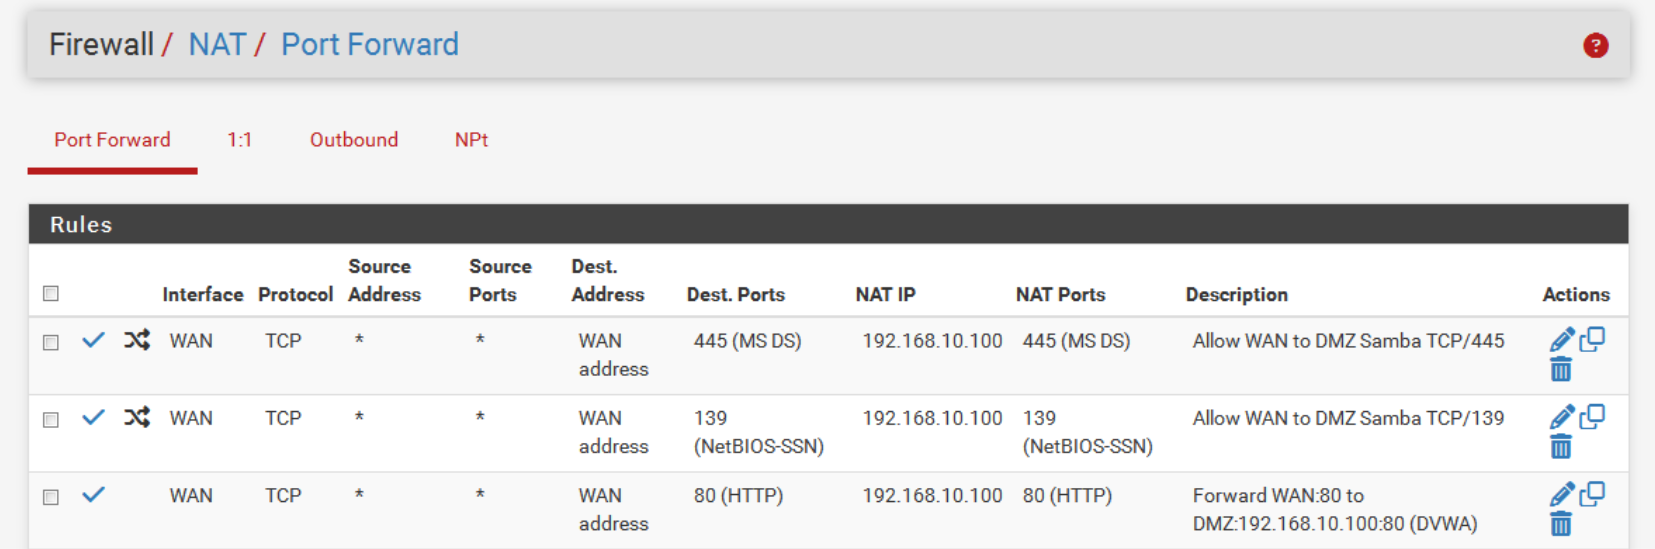
\includegraphics[width=0.9\textwidth]{screenshots/nat-rules.png}
		}{
			\includegraphics[width=0.9\textwidth]{example-image}
			\caption*{\textbf{Attention :} Fichier screenshots/nat-rules.png introuvable.}
		}
		\caption{Configuration des règles NAT Port Forward sur pfSense}
		\label{fig:nat-screenshot}
	\end{figure}
	
	\section{Règles de Pare-Feu WAN}
	Les règles automatiquement générées ont été vérifiées et placées en haut de la pile de filtrage. Elles autorisent explicitement le trafic entrant sur les ports spécifiés vers la DMZ.
	
	\begin{lstlisting}[caption=Règles de Pare-Feu WAN (Extrait)]
		Pass | TCP | Any | WAN address | 80  | Allow WAN to DMZ Web
		Pass | TCP | Any | WAN address | 139 | Allow WAN to DMZ Samba
		Pass | TCP | Any | WAN address | 445 | Allow WAN to DMZ SMB
	\end{lstlisting}
	
	\begin{figure}[H]
		\centering
		\IfFileExists{screenshots/firewall-rules.png}{
			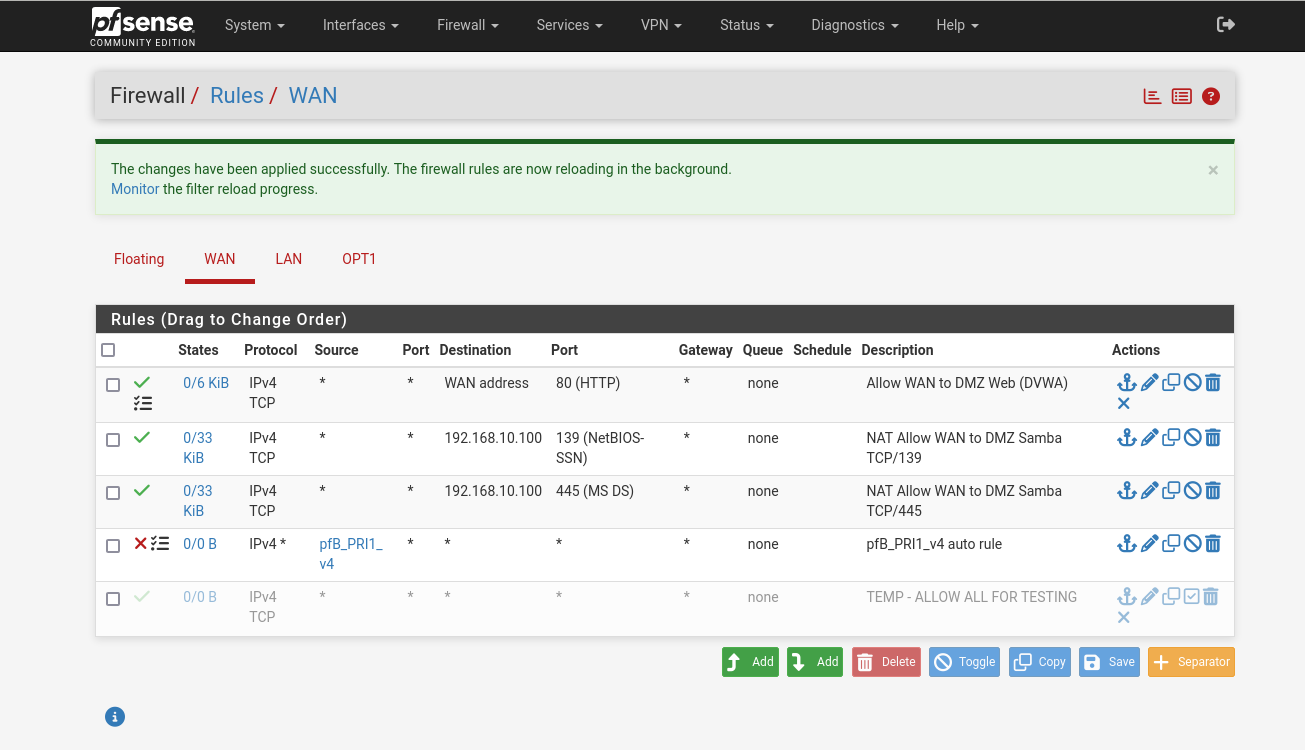
\includegraphics[width=0.9\textwidth]{screenshots/firewall-rules.png}
		}{
			\includegraphics[width=0.9\textwidth]{example-image}
			\caption*{\textbf{Attention :} Fichier screenshots/firewall-rules.png introuvable.}
		}
		\caption{Règles de Pare-Feu WAN associées au NAT}
		\label{fig:firewall-screenshot}
	\end{figure}
	
	\section{Déblocage des Réseaux Privés (Laboratoire)}
	\textbf{Configuration critique pour le laboratoire :} L'option \texttt{Block private networks and loopback addresses} sur l'interface WAN a été \textbf{désactivée}.
	\begin{lstlisting}[caption=Désactivation dans les paramètres de l'interface WAN]
		Interfaces > WAN > Reserved Networks
		[ ] Block private networks and loopback addresses
		[ ] Block bogon networks
	\end{lstlisting}
	\textbf{Justification :} Cette option est activée par défaut pour bloquer les adresses IP privées (RFC 1918) sur l'interface WAN. Dans ce laboratoire, la machine attaquante (Parrot Security) utilise une IP privée (192.168.100.150) via VMware NAT. La désactivation est nécessaire pour permettre les tests. \textbf{Ne JAMAIS faire cela en production.}
	
	% ------------------------------------------------------------------------------
	% CHAPITRE 4 : SÉCURITÉ AVANCÉE
	% ------------------------------------------------------------------------------
	\chapter{Sécurité Avancée : pfBlockerNG et Snort}
	
	\section{pfBlockerNG : Intelligence sur les Menaces}
	pfBlockerNG a été installé via le gestionnaire de packages pour fournir une couche de sécurité basée sur le renseignement.
	
	\subsection{Configuration des Feeds}
	\begin{itemize}
		\item \textbf{IPv4 Blocklists :} Activation des listes \textit{pfB\_PRI1\_v4}.
		\item \textbf{GeoIP :} Configuration avec MaxMind (nécessite une clé API).
		\item \textbf{DNSBL :} Activé pour bloquer les domaines malveillants au niveau DNS.
	\end{itemize}
	
	\subsection{Statistiques de Blocage}
	Au moment de la rédaction, pfBlockerNG bloque activement plus de 1400 adresses IP malveillantes connues.
	\begin{lstlisting}[caption=Statut pfBlockerNG Dashboard]
		pfB_PRI1_v4 : 1,458 IPs bloquées
		DNSBL       : 0 Requêtes bloquées (Test initial)
	\end{lstlisting}
	
	\subsection{Liste d'Exception (Suppression List)}
	Pour permettre à la machine attaquante de tester l'infrastructure sans être bloquée par les listes noires, son IP a été ajoutée à la liste de suppression.
	\begin{lstlisting}[caption=Configuration Suppression List]
		IPv4 Suppression :
		192.168.100.150/32  # Lab Attacker (Parrot) - Allow
	\end{lstlisting}
	
	\section{Snort : Détection d'Intrusion (IDS)}
	Snort a été déployé sur l'interface WAN pour surveiller le trafic entrant en temps réel.
	
	\subsection{Règles Activées}
	\begin{itemize}
		\item Emerging Threats (ET) Open Rules.
		\item Snort VRT Rules (Community).
		\item Categories : Scan Detection, Exploit Kits, Malware C\&C.
	\end{itemize}
	
	\subsection{Exemple d'Alerte}
	Lors des scans Nmap, Snort a généré des alertes pertinentes.
	\begin{lstlisting}[caption=Exemple d'alerte Snort]
		[Priority: 3] ET SCAN Suspicious inbound to mySQL port 3306
		Source      : 192.168.100.150:58890
		Destination : 192.168.100.6:3306
		Action      : Alert Only (Mode IDS)
	\end{lstlisting}
	
	% ------------------------------------------------------------------------------
	% CHAPITRE 5 : SÉCURITÉ DES HÔTES
	% ------------------------------------------------------------------------------
	\chapter{Sécurité au Niveau de l'Hôte (Ubuntu DMZ)}
	
	\section{UFW : Pare-feu Applicatif}
	Un pare-feu local (Uncomplicated Firewall) a été configuré sur le serveur Ubuntu pour contrôler les connexions entrantes au niveau du kernel.
	
	\begin{lstlisting}[caption=Configuration UFW sur Ubuntu DMZ]
		$ sudo ufw status numbered
		Status: active
		
		[ 1] 22/tcp                ALLOW IN    Anywhere
		[ 2] 80/tcp                ALLOW IN    Anywhere
		[ 3] 139/tcp               ALLOW IN    Anywhere
		[ 4] 445/tcp               ALLOW IN    Anywhere
		[ 5] 22/tcp (v6)           ALLOW IN    Anywhere (v6)
		[ 6] 80/tcp (v6)           ALLOW IN    Anywhere (v6)
		[ 7] 139/tcp (v6)          ALLOW IN    Anywhere (v6)
		[ 8] 445/tcp (v6)          ALLOW IN    Anywhere (v6)
	\end{lstlisting}
	\textbf{Rationale :} UFW agit comme une barrière supplémentaire. Même si le pare-feu pfSense est compromis ou mal configuré, l'hôte reste protégé par ses propres règles.
	
	\section{Fail2Ban : Protection contre le Brute-Force}
	Fail2Ban surveille les logs d'authentification pour bannir les IP suspectes.
	
	\begin{lstlisting}[caption=Configuration Fail2Ban (jail.local)]
		[sshd]
		enabled  = true
		port     = ssh
		filter   = sshd
		logpath  = /var/log/auth.log
		maxretry = 3
		bantime  = 600
		findtime = 600
	\end{lstlisting}
	
	\section{Conteneurisation des Services}
	Les services vulnérables sont exécutés dans des conteneurs Docker pour limiter l'impact d'une compromission.
	
	\begin{lstlisting}[caption=Conteneurs Actifs sur Ubuntu DMZ]
		$ sudo docker ps
		CONTAINER ID   IMAGE                    STATUS       PORTS                    NAMES
		5b1166370a66   ghcr.io/digininja/dvwa   Up 6 hours   0.0.0.0:80->80/tcp       dvwa
		5944e93265e3   dperson/samba            Up 6 hours   0.0.0.0:139->139/tcp,    samba
		0.0.0.0:445->445/tcp
	\end{lstlisting}
	
	% ------------------------------------------------------------------------------
	% CHAPITRE 6 : ANALYSE DES LOGS
	% ------------------------------------------------------------------------------
	\chapter{Analyse des Journaux et Validation}
	
	\section{Méthodologie d'Analyse}
	Les journaux du pare-feu pfSense (\texttt{Status > System Logs > Firewall}) ont été exportés et analysés pour valider le comportement des règles de sécurité. L'objectif était d'identifier les trafics autorisés, les trafics bloqués et les erreurs de configuration.
	
	\section{Phase 1 : Trafic Autorisé (Before 22:33)}
	Entre 22:13 et 22:25, les logs montrent que le trafic de l'attaquant vers la DMZ est correctement autorisé par la règle \texttt{(12004)}.
	
	\begin{table}[ht]
		\centering
		\small
		\renewcommand{\arraystretch}{1.4}
		\setlength{\arrayrulewidth}{0.5pt}
		\begin{tabular}{p{2.4cm} p{4.2cm} p{3.6cm} >{\centering\arraybackslash}p{1.8cm} >{\centering\arraybackslash}p{1.8cm}}
			\arrayrulecolor{tableborder}
			\hline
			\tableheadcolor
			\textcolor{tableheadfg}{\textbf{Timestamp}} &
			\textcolor{tableheadfg}{\textbf{Source}} &
			\textcolor{tableheadfg}{\textbf{Destination}} &
			\textcolor{tableheadfg}{\textbf{Rule}} &
			\textcolor{tableheadfg}{\textbf{Action}} \\
			\hline
			\rowcolor{tablerowalt}
			22:13:57 & 192.168.100.150:38056 & 192.168.10.100:80  & (12004) & \textcolor{green!50!black}{\textbf{ALLOW}} \\
			22:15:21 & 192.168.100.150:44838 & 192.168.10.100:139 & (12004) & \textcolor{green!50!black}{\textbf{ALLOW}} \\
			\rowcolor{tablerowalt}
			22:25:57 & 192.168.100.150:38414 & 192.168.10.100:80  & (12004) & \textcolor{green!50!black}{\textbf{ALLOW}} \\
			\hline
		\end{tabular}
		\caption{Logs de Trafic Autorisé (Phase 1)}
		\label{tab:logs-allow}
	\end{table}
	
	\section{Phase 2 : Erreur de Configuration NAT (Port 445)}
	Durant la phase de test initiale, une erreur de frappe dans la règle NAT a été identifiée grâce aux logs. Le trafic était redirigé vers une IP incorrecte.
	
	\begin{lstlisting}[style=logstyle,caption=Preuve de l'erreur NAT dans les logs]
		Mar 2 22:15:19 WAN (12004) 192.168.100.150:59708 -> 129.168.10.100:445 TCP:S
		Mar 2 22:15:20 WAN (12004) 192.168.100.150:59708 -> 129.168.10.100:445 TCP:S
		Mar 2 22:15:28 WAN (12004) 192.168.100.150:59858 -> 129.168.10.100:445 TCP:S
	\end{lstlisting}
	\textbf{Analyse :} L'adresse de destination devrait être \texttt{192.168.10.100}. L'adresse \texttt{129.168.10.100} est invalide dans ce contexte (faute de frappe : \texttt{129} au lieu de \texttt{192}). Cette erreur a été corrigée dans la configuration NAT.
	
	\section{Phase 3 : Blocage par Default Deny (After 22:33)}
	Après modification des règles de pare-feu (désactivation de la règle temporaire "Allow All"), le trafic a commencé à être bloqué par la règle par défaut, indiquant que les règles spécifiques n'étaient pas correctement appariées.
	
	\begin{table}[ht]
		\centering
		\small
		\renewcommand{\arraystretch}{1.4}
		\setlength{\arrayrulewidth}{0.5pt}
		\begin{tabular}{p{2.2cm} p{4.2cm} p{3.4cm} p{3.4cm} >{\centering\arraybackslash}p{1.6cm}}
			\arrayrulecolor{tableborder}
			\hline
			\tableheadcolor
			\textcolor{tableheadfg}{\textbf{Timestamp}} &
			\textcolor{tableheadfg}{\textbf{Source}} &
			\textcolor{tableheadfg}{\textbf{Destination}} &
			\textcolor{tableheadfg}{\textbf{Rule}} &
			\textcolor{tableheadfg}{\textbf{Action}} \\
			\hline
			\rowcolor{tablerowalt}
			22:33:21 & 192.168.100.150:38484 & 192.168.10.100:80 & Default deny & \textcolor{accent}{\textbf{BLOCK}} \\
			22:34:28 & 192.168.100.150:38492 & 192.168.10.100:80 & Default deny & \textcolor{accent}{\textbf{BLOCK}} \\
			\rowcolor{tablerowalt}
			22:50:53 & 192.168.100.150:38598 & 192.168.10.100:80 & Default deny & \textcolor{accent}{\textbf{BLOCK}} \\
			\hline
		\end{tabular}
		\caption{Logs de Trafic Bloqué (Phase 3)}
		\label{tab:logs-deny}
	\end{table}
	
	\textbf{Résolution :} Les règles de pare-feu WAN ont été recréées en utilisant l'option \textit{Add associated filter rule} lors de la configuration NAT, garantissant ainsi que la destination corresponde correctement à l'adresse WAN avant translation.
	
	\section{Validation Finale}
	Après correction, les tests de connectivité depuis la machine Parrot Security confirment le fonctionnement :
	\begin{lstlisting}[caption=Tests de Connectivité depuis l'Attaquant (Parrot)]
		$ curl -I http://192.168.100.6
		HTTP/1.1 301 Moved Permanently
		Server: nginx
		
		$ nc -zv 192.168.100.6 139
		Ncat: Connected to 192.168.100.6:139.
		
		$ nc -zv 192.168.100.6 445
		Ncat: Connected to 192.168.100.6:445.
	\end{lstlisting}
	
	% ------------------------------------------------------------------------------
	% CHAPITRE 7 : RÉPONSES AUX QUESTIONS DE RÉFLEXION
	% ------------------------------------------------------------------------------
	\chapter{Réponses aux Questions de Réflexion}
	
	\section{Question 1 : Importance de la Segmentation Réseau}
	
	\subsection{Définition et Principe Stratégique}
	La segmentation réseau est un principe fondamental de la \textit{défense en profondeur} qui consiste à diviser l'infrastructure en zones de confiance distinctes, chacune ayant des politiques de sécurité et des contrôles d'accès spécifiques.
	
	\subsection{Importance Stratégique}
	\begin{enumerate}
		\item \textbf{Limitation du \textit{Blast Radius} :} 
		Si un attaquant compromise une machine dans la DMZ (ex: notre serveur Ubuntu), il ne peut pas accéder directement au LAN. Dans notre laboratoire, même si l'attaquant Parrot Security parvient à exploiter le serveur web DVWA, il restera confiné à la zone DMZ car pfSense bloque par défaut le routage DMZ → LAN.
		
		\item \textbf{Application du Principe du Moindre Privilège :} 
		Chaque zone a des politiques d'accès spécifiques. Les services publics (HTTP, SMB) sont exposés uniquement depuis la DMZ, tandis que le LAN reste strictement isolé.
		
		\item \textbf{Conformité Réglementaire :} 
		Les standards tels que PCI-DSS (Payment Card Industry), RGPD, et ISO 27001 exigent l'isolation des données sensibles dans des segments réseau dédiés.
		
		\item \textbf{Surveillance et Audit Simplifiés :} 
		Chaque zone dispose de points de contrôle uniques (interfaces pfSense), facilitant l'analyse des logs et la détection d'anomalies.
	\end{enumerate}
	
	\subsection{Risques sans Segmentation}
	Dans un réseau plat (sans segmentation), les conséquences d'une compromission sont catastrophiques :
	
	\begin{itemize}
		\item \textbf{Propagation Latérale Illimitée :} L'attaquant peut scanner et attaquer toutes les machines du réseau sans restriction.
		\item \textbf{Compromission en Cascade :} Une vulnérabilité sur un serveur web expose directement les contrôleurs de domaine, bases de données et postes utilisateurs.
		\item \textbf{Absence de Point de Contrôle :} Aucune visibilité sur les flux inter-machines, rendant la détection d'intrusion impossible.
	\end{itemize}
	
	\subsection{Exemple Concret de Notre Laboratoire}
	\begin{itemize}
		\item \textbf{Avec segmentation :} Le trafic de Parrot (192.168.100.150) peut atteindre Ubuntu DMZ (192.168.10.100) via NAT, mais ne peut \textbf{PAS} atteindre directement Windows Client (192.168.20.50) car pfSense bloque par défaut le routage inter-zones.
		\item \textbf{Sans segmentation :} L'attaquant pourrait directement exploiter Windows XP (système obsolète) depuis Internet.
	\end{itemize}
	
	\textbf{Citation pertinente :} \textit{"Security is a journey, not a destination. Network segmentation is the roadmap."} --- Bruce Schneier.
	
	% ------------------------------------------------------------------------------
	\section{Question 2 : Rôle Principal de pfSense}
	
	pfSense agit comme le \textbf{point de contrôle central} de notre architecture, assurant à la fois le routage, le filtrage et les services réseau essentiels.
	
	\subsection{Fonctions Principales}
	
	\subsubsection{1. Routeur Inter-Zones}
	\begin{itemize}
		\item Route le trafic entre WAN (192.168.100.0/24), DMZ (192.168.10.0/24) et LAN (192.168.20.0/24).
		\item Chaque zone utilise pfSense comme passerelle par défaut :
		\begin{itemize}
			\item Ubuntu DMZ → Gateway : 192.168.10.1
			\item Windows Client → Gateway : 192.168.20.1
		\end{itemize}
	\end{itemize}
	
	\subsubsection{2. Pare-feu Stateful}
	\begin{itemize}
		\item Applique des règles de filtrage par interface (WAN/DMZ/LAN).
		\item Maintient une \textit{table d'états} des connexions (stateful inspection) pour suivre les sessions TCP/UDP.
		\item Politique par défaut : \textbf{"Default Deny"} --- tout ce qui n'est pas explicitement autorisé est bloqué (voir Chapitre 6, Phase 3).
	\end{itemize}
	
	\subsubsection{3. NAT/PAT (Network Address Translation)}
	\begin{itemize}
		\item \textbf{Port Forwarding :} Expose les services DMZ (80, 139, 445) vers le WAN tout en masquant la topologie interne.
		\item \textbf{Translation d'adresses :} Masque les adresses IP privées derrière l'adresse WAN publique, protégeant contre le fingerprinting réseau.
	\end{itemize}
	
	\subsubsection{4. Services Réseau Essentiels}
	\begin{itemize}
		\item \textbf{DHCP Server :} Attribution automatique d'IPs dans DMZ (.10-.50) et LAN (.10-.50), simplifiant l'administration.
		\item \textbf{DNS Resolver :} Résolution de noms pour les clients internes, avec possibilité de filtrage DNS via pfBlockerNG DNSBL.
	\end{itemize}
	
	\subsection{Contribution à la Sécurité Globale}
	\begin{enumerate}
		\item \textbf{Visibilité Complète :} Logs détaillés de tous les flux réseau (voir Chapitre 6).
		\item \textbf{Point de Contrôle Unique :} Facilite l'audit et l'application de politiques de sécurité centralisées.
		\item \textbf{Extensibilité :} Support IDS/IPS via packages (Snort), intelligence sur les menaces (pfBlockerNG), VPN, etc.
		\item \textbf{Résilience :} Architecture \textit{fail-secure} --- en cas de panne, tout trafic est bloqué par défaut.
	\end{enumerate}
	
	% ------------------------------------------------------------------------------
	\section{Question 3 : Déblocage des Réseaux Privés sur WAN}
	
	\subsection{Mécanisme de Blocage par Défaut}
	Par défaut, pfSense active l'option \texttt{Block private networks and loopback addresses} sur l'interface WAN. Cette option bloque automatiquement tout trafic entrant provenant de plages RFC 1918 :
	\begin{itemize}
		\item 10.0.0.0/8
		\item 172.16.0.0/12
		\item 192.168.0.0/16
	\end{itemize}
	
	\subsection{Justification Technique}
	\textbf{En production}, ces adresses ne devraient \textbf{JAMAIS} apparaître sur l'interface WAN car elles ne sont pas routables sur Internet public. Leur présence indiquerait :
	\begin{itemize}
		\item \textbf{Attaque de Spoofing :} Un attaquant usurpe une adresse IP privée pour contourner les règles de filtrage basées sur la géolocalisation.
		\item \textbf{Mauvaise Configuration FAI :} Le fournisseur d'accès Internet a mal configuré son routage (rare mais possible).
		\item \textbf{Tentative de Rebond :} Utilisation d'adresses privées pour dissimuler l'origine réelle de l'attaque.
	\end{itemize}
	
	\subsection{Pourquoi Désactiver dans Notre Laboratoire}
	Notre machine attaquante (Parrot Security) utilise une IP privée \textbf{192.168.100.150} via VMware NAT. Sans désactivation de cette option, pfSense rejetterait \textbf{tous les paquets} provenant de cette source \textbf{avant même} d'évaluer les règles de pare-feu et NAT.
	
	\textbf{Conséquence :} Les tests de pénétration seraient impossibles car le trafic serait bloqué silencieusement.
	
	\subsection{Implications en Production}
	\begin{tcolorbox}[colback=accent!5!white, colframe=accent, title=\textbf{AVERTISSEMENT CRITIQUE}]
		\textbf{NE JAMAIS désactiver cette protection en production !}
		
		Désactiver cette option exposerait le réseau à :
		\begin{itemize}
			\item \textbf{Attaques par Rebond :} Contournement des listes de blocage basées sur IP publiques.
			\item \textbf{Usurpation d'Identité :} Un attaquant pourrait se faire passer pour un système interne.
			\item \textbf{Risque de Routage Asymétrique :} Paquets retours non tracés, causant des failles dans l'audit de sécurité.
		\end{itemize}
	\end{tcolorbox}
	
	\subsection{Preuve dans Nos Logs}
	Référence Chapitre 3, Section 3.5 : Après désactivation, le trafic de 192.168.100.150 est désormais évalué par les règles NAT/Firewall au lieu d'être rejeté en amont.
	
	% ------------------------------------------------------------------------------
	\section{Question 4 : Modes de Carte Réseau (VMware/VirtualBox)}
	
	Bien que nous ayons utilisé VMware, les concepts sont identiques à VirtualBox.
	
	\subsection{Tableau Comparatif}
	
	\begin{table}[H]
		\centering
		\small
		\renewcommand{\arraystretch}{1.8}
		\setlength{\arrayrulewidth}{0.5pt}
		\begin{tabular}{p{3.5cm} p{5cm} p{6cm}}
			\arrayrulecolor{tableborder}
			\hline
			\tableheadcolor
			\textcolor{tableheadfg}{\textbf{Mode}} &
			\textcolor{tableheadfg}{\textbf{Description}} &
			\textcolor{tableheadfg}{\textbf{Cas d'usage dans notre lab}} \\
			\hline
			\rowcolor{tablerowalt}
			\textbf{NAT} & 
			VM obtient une IP privée via DHCP de l'hyperviseur. Peut accéder à Internet via translation. Les VMs en NAT ne se voient pas entre elles. &
			\textbf{Parrot Security :} Simule un attaquant externe avec accès Internet tout en étant isolé des autres VMs. IP : 192.168.100.150 \\
			
			\textbf{Bridged (Accès par pont)} &
			VM connectée directement au réseau physique de l'hôte. Obtient une IP du routeur physique. &
			Alternative pour pfSense WAN si on veut tester depuis d'autres machines physiques du réseau local. \\
			
			\rowcolor{tablerowalt}
			\textbf{Internal Network (Réseau interne)} &
			VMs connectées au même réseau interne peuvent communiquer entre elles, mais sont isolées du reste. Pas d'accès Internet ni au réseau hôte. &
			\textbf{DMZ\_SEG et LAN\_SEG :} Crée une isolation stricte. Seul pfSense fait le pont entre ces segments. \\
			\hline
		\end{tabular}
		\caption{Comparaison des Modes de Carte Réseau}
	\end{table}
	
	\subsection{Exemple Concret}
	\begin{lstlisting}[caption=Isolation Réseau Vérifiée]
		# Parrot (NAT) -> peut pinger 8.8.8.8 et l'IP WAN de pfSense
		$ ping 8.8.8.8            # OK
		$ ping 192.168.100.6      # OK (WAN pfSense)
		
		# Ubuntu DMZ (LAN Segment: DMZ_SEG) -> isolation stricte
		$ ping 8.8.8.8            # FAIL (pas d'acces direct Internet)
		$ ping 192.168.10.1       # OK (pfSense DMZ gateway)
		$ ping 192.168.20.1       # FAIL (pas de routage DMZ->LAN)
		
		# Windows Client (LAN Segment: LAN_SEG) -> isolation maximale
		$ ping 192.168.20.1       # OK (pfSense LAN gateway)
		$ ping 192.168.10.100     # FAIL (pas de routage LAN->DMZ sans regle)
	\end{lstlisting}
	
	Cette isolation est la \textbf{clé} de notre segmentation réseau.
	
	% ------------------------------------------------------------------------------
	\section{Question 5 : Dépannage DHCP}
	
	\subsection{Scénario}
	La machine DMZ (Ubuntu) ne parvient pas à obtenir une adresse IP via DHCP après configuration initiale.
	
	\subsection{Méthodologie de Dépannage Systématique}
	
	\subsubsection{Étape 1 : Vérifier la Configuration Réseau de la VM}
	\begin{lstlisting}[caption=Diagnostic Réseau sur Ubuntu DMZ]
		# Vérifier l'état de l'interface
		$ ip link show
		# L'interface doit être UP (ex: eth0: <BROADCAST,MULTICAST,UP>)
		
		# Forcer une requête DHCP en verbose
		$ sudo dhclient -v eth0
		# Observer si DHCPDISCOVER est envoyé et si DHCPOFFER est reçu
		
		# Vérifier les logs système
		$ sudo journalctl -u NetworkManager -f
	\end{lstlisting}
	\textbf{Pourquoi ?} Si l'interface est DOWN ou le service network-manager inactif, aucune requête DHCP ne sera envoyée vers pfSense.
	
	\subsubsection{Étape 2 : Vérifier le Service DHCP sur pfSense}
	\begin{enumerate}
		\item Interface web : \texttt{Services > DHCP Server > DMZ}
		\item Vérifier que \textbf{"Enable"} est coché
		\item Vérifier la plage : 192.168.10.10 -- 192.168.10.50
		\item Vérifier qu'il n'y a pas de conflit de plage (ex: réservations statiques hors pool)
		\item Consulter les logs : \texttt{Status > System Logs > DHCP}
	\end{enumerate}
	\textbf{Pourquoi ?} Si le serveur DHCP est désactivé ou mal configuré, aucune offre (DHCPOFFER) ne sera envoyée.
	
	\subsubsection{Étape 3 : Vérifier la Connectivité Réseau VMware}
	\begin{itemize}
		\item \textbf{Paramètres VM Ubuntu :} Adaptateur bien sur \textit{"Custom: DMZ\_SEG"} ?
		\item \textbf{Virtual Network Editor :} DMZ\_SEG existe et est de type \textit{"LAN Segment"} ?
		\item \textbf{Cable Connected :} La case \textit{"Connect at power on"} est cochée ?
	\end{itemize}
	\textbf{Pourquoi ?} Si la VM n'est pas sur le bon segment virtuel, elle ne peut physiquement pas atteindre l'interface em1 de pfSense.
	
	\subsubsection{Étape 4 : Capture de Paquets (Diagnostic Avancé)}
	\begin{lstlisting}[caption=Analyse DHCP avec tcpdump sur pfSense]
		# Sur pfSense (via SSH ou console)
		$ tcpdump -i em1 port 67 or port 68 -vvv
		
		# Observer :
		# - DHCP Discover (client → serveur, port 68 → 67)
		# - DHCP Offer   (serveur → client, port 67 → 68)
		# - DHCP Request (client → serveur)
		# - DHCP Ack     (serveur → client)
	\end{lstlisting}
	Cela permet d'identifier précisément où la communication échoue :
	\begin{itemize}
		\item \textbf{Pas de DISCOVER :} Problème client (interface DOWN, pas de câble virtuel).
		\item \textbf{DISCOVER visible mais pas d'OFFER :} Problème serveur DHCP pfSense.
		\item \textbf{OFFER visible mais pas de REQUEST :} Client refuse l'offre (config IP statique concurrente).
	\end{itemize}
	
	\subsubsection{Étape 5 : Vérifier les Règles Firewall}
	Aller dans \texttt{Firewall > Rules > DMZ} et vérifier qu'aucune règle ne bloque le trafic UDP 67/68 (DHCP).
	
	\textbf{Note :} Par défaut, pfSense autorise tout trafic sortant des interfaces internes (DMZ, LAN), donc ce cas est rare, mais peut arriver après modification manuelle.
	
	% ------------------------------------------------------------------------------
	\section{Question 6 : Intérêt Pédagogique des Erreurs Simulées}
	
	\subsection{Philosophie de l'Apprentissage par l'Erreur}
	L'introduction délibérée d'erreurs dans un environnement de laboratoire est une méthode pédagogique éprouvée, basée sur le principe \textit{"Learning by Debugging"}. Elle développe des compétences critiques en analyse forensique et dépannage système.
	
	\subsection{Erreurs Rencontrées dans Notre TP}
	
	\subsubsection{1. Désactivation du Blocage RFC1918 (Chapitre 3, Section 3.5)}
	\begin{itemize}
		\item \textbf{Intérêt :} Comprendre les mécanismes de protection périmétrique et leurs implications.
		\item \textbf{Apprentissage :} Distinction claire entre environnement lab et production.
		\item \textbf{Réflexion Critique :} \textit{"Pourquoi cette sécurité existe-t-elle ? Quels sont les risques si je la désactive ?"}
	\end{itemize}
	
	\subsubsection{2. Erreur NAT Découverte (Chapitre 6, Phase 2)}
	\textbf{Erreur :} Typo dans la règle NAT → destination \texttt{129.168.10.100} au lieu de \texttt{192.168.10.100}.
	
	\begin{itemize}
		\item \textbf{Intérêt :} Apprendre à lire et interpréter les logs firewall.
		\item \textbf{Compétence Développée :} Méthodologie de dépannage systématique (bottom-up analysis).
		\item \textbf{Réalisme :} En production, ce type de typo est fréquent et peut causer des incidents majeurs.
	\end{itemize}
	
	\subsubsection{3. Blocage par "Default Deny" après Modification (Chapitre 6, Phase 3)}
	\begin{itemize}
		\item \textbf{Intérêt :} Comprendre l'ordre d'évaluation des règles de pare-feu.
		\item \textbf{Apprentissage :} Différence entre règles NAT et règles Firewall, importance du matching correct.
		\item \textbf{Meilleure Pratique :} Toujours utiliser \textit{"Add associated filter rule"} lors de la création de règles NAT.
	\end{itemize}
	
	\subsection{Bénéfices Globaux}
	\begin{enumerate}
		\item \textbf{Développement de l'Esprit Critique :} Remettre en question chaque configuration, comprendre le \textit{"pourquoi"}.
		\item \textbf{Simulation de Situations Réelles :} Les erreurs de production sont rarement documentées dans les manuels. Cette approche prépare aux incidents réels.
		\item \textbf{Renforcement par l'Expérience Pratique :} On retient 90\% de ce qu'on fait et corrige, contre 10\% de ce qu'on lit passivement.
		\item \textbf{Compréhension Profonde :} Comprendre un système par ses échecs permet d'anticiper les problèmes futurs.
	\end{enumerate}
	
	\textbf{Citation :} 
	\begin{quote}
		\textit{"I have not failed. I've just found 10,000 ways that won't work."}\\
		--- Thomas Edison
	\end{quote}
	
	En cybersécurité, comprendre les échecs est aussi important que réussir. Les erreurs sont des opportunités d'apprentissage, pas des obstacles.
	
	% ------------------------------------------------------------------------------
	\section{Question 7 : Tableau Récapitulatif des Adresses IP}
	
	\begin{table}[H]
		\centering
		\renewcommand{\arraystretch}{1.5}
		\setlength{\arrayrulewidth}{0.5pt}
		\begin{tabular}{p{5cm} >{\centering\arraybackslash}p{4cm} >{\centering\arraybackslash}p{4.5cm}}
			\arrayrulecolor{tableborder}
			\hline
			\tableheadcolor
			\textcolor{tableheadfg}{\textbf{Machine}} &
			\textcolor{tableheadfg}{\textbf{Adresse IP}} &
			\textcolor{tableheadfg}{\textbf{Passerelle}} \\
			\hline
			\rowcolor{tablerowalt}
			pfSense (WAN) & 192.168.100.6 (DHCP) & 192.168.100.2 (VMware Gateway) \\
			
			pfSense (DMZ) & 192.168.10.1 (Statique) & N/A (interface locale) \\
			
			\rowcolor{tablerowalt}
			pfSense (INTERNAL\_LAN) & 192.168.20.1 (Statique) & N/A (interface locale) \\
			
			Ubuntu DMZ (Metasploitable équivalent) & 192.168.10.100 (Statique) & 192.168.10.1 (pfSense DMZ) \\
			
			\rowcolor{tablerowalt}
			Windows Client & 192.168.20.50 (DHCP) & 192.168.20.1 (pfSense LAN) \\
			
			Parrot Security (Kali équivalent) & 192.168.100.150 (DHCP) & 192.168.100.2 (VMware Gateway) \\
			\hline
		\end{tabular}
		\caption{Tableau Récapitulatif des Adresses IP et Passerelles}
		\label{tab:ip-summary}
	\end{table}
	
	\subsection{Notes Importantes}
	\begin{itemize}
		\item \textbf{Adresses DHCP :} Les adresses attribuées par DHCP (Windows Client, Parrot) peuvent varier entre les redémarrages si aucune réservation statique n'est configurée.
		
		\item \textbf{Passerelles pfSense :} Les interfaces DMZ et LAN de pfSense n'ont pas de passerelle car ce sont des réseaux locaux dont pfSense est le \textit{maître}. Seule l'interface WAN a une passerelle (simulant le FAI).
		
		\item \textbf{Équivalence Terminologique :} Bien que nous ayons utilisé Ubuntu au lieu de Metasploitable et Parrot au lieu de Kali, les fonctions réseau sont identiques (cible DMZ et attaquant WAN respectivement).
	\end{itemize}
	
	% ------------------------------------------------------------------------------
	% CHAPITRE 8 : Conclusion et Perspectives
	% ------------------------------------------------------------------------------
	
	\chapter{Conclusion et Perspectives}
	
	\section{Synthèse des Résultats}
	Ce projet a permis de déployer une infrastructure réseau complexe et sécurisée, intégrant des technologies clés en cybersécurité :
	\begin{itemize}
		\item Segmentation réseau stricte (WAN, DMZ, LAN) via VMware.
		\item Pare-feu périmétrique configuré avec des règles NAT et Filter précises.
		\item Intelligence sur les menaces via pfBlockerNG.
		\item Détection d'intrusion via Snort.
		\item Sécurité hôte renforcée (UFW, Fail2Ban, Docker).
	\end{itemize}
	
	Les tests de connectivité ont confirmé que les services exposés (HTTP, SMB) sont accessibles depuis le WAN tout en étant protégés par les multiples couches de sécurité. L'analyse des logs a permis d'identifier et de corriger des erreurs de configuration critiques (typo NAT, règles firewall mismatch).
	
	\section{Difficultés Rencontrées}
	\begin{enumerate}
		\item \textbf{Correspondance des Règles Firewall :} La compréhension du moment où pfSense évalue les règles (avant ou après NAT) a nécessité plusieurs itérations. L'utilisation de règles associées automatiques a résolu le problème.
		\item \textbf{Blocage RFC1918 :} La nécessité de désactiver le blocage des réseaux privés sur le WAN pour le laboratoire a été un point de vigilance important pour ne pas l'appliquer en production.
		\item \textbf{Filtrage SMB :} Les ports 139/445 ont montré des états "filtered" lors des scans Nmap malgré une connexion TCP réussie (nc), probablement dû à la gestion des états FIN/ACK par le pare-feu.
	\end{enumerate}
	
	\section{Perspectives d'Amélioration}
	Pour aller plus loin, les axes suivants pourraient être explorés :
	\begin{itemize}
		\item Mise en place de VLANs pour isoler davantage le trafic au sein de VMware.
		\item Configuration de Snort en mode IPS (Inline Blocking) pour bloquer activement les attaques.
		\item Intégration d'un SIEM (ex: ELK Stack) pour centraliser et corréler les logs de pfSense, Snort et des hôtes.
		\item Automatisation du déploiement via Ansible ou Terraform.
	\end{itemize}
	
	% ------------------------------------------------------------------------------
	% BIBLIOGRAPHIE
	% ------------------------------------------------------------------------------
	\begin{thebibliography}{99}
		
		\bibitem{cisco-segmentation}
		Cisco Systems. \textit{What Is Network Segmentation?}. Cisco, 2024. Consulté sur \url{https://www.cisco.com/c/en/us/products/security/what-is-network-segmentation.html}
		
		\bibitem{netgate-pfsense}
		Netgate. \textit{pfSense Documentation}. Netgate, 2024. Consulté sur \url{https://docs.netgate.com/pfsense/en/latest/}
		
		\bibitem{netgate-nat}
		Netgate. \textit{NAT Port Forward}. Netgate Documentation, 2024. Consulté sur \url{https://docs.netgate.com/pfsense/en/latest/nat/port-forwards.html}
		
		\bibitem{rfc1918}
		Rekhter, Y., Moskowitz, B., Karrenberg, D., de Groot, G. J., et Lear, E. \textit{Address Allocation for Private Internets}. RFC 1918, IETF, février 1996. Consulté sur \url{https://www.rfc-editor.org/rfc/rfc1918}
		
		\bibitem{snort-org}
		Cisco Talos. \textit{Snort 3 User Manual}. Snort.org, 2024. Consulté sur \url{https://www.snort.org/documents}
		
		\bibitem{pfblockerng}
		Netgate Forums. \textit{pfBlockerNG-devel Documentation and FAQ}. pfSense Forum, 2024. Consulté sur \url{https://forum.netgate.com/topic/114116/pfblockerng-devel}
		
		\bibitem{ufw-man}
		Ubuntu Community Help Wiki. \textit{Uncomplicated Firewall (UFW)}. Ubuntu, 2024. Consulté sur \url{https://help.ubuntu.com/community/UFW}
		
		\bibitem{fail2ban-doc}
		Fail2Ban Project. \textit{Fail2Ban Documentation}. Consulté sur \url{https://fail2ban.readthedocs.io/en/latest/}
		
		\bibitem{docker-docs}
		Docker Inc. \textit{Docker Documentation}. Consulté sur \url{https://docs.docker.com}
		
		\bibitem{dvwa}
		DVWA Project. \textit{Damn Vulnerable Web Application (DVWA)}. GitHub, 2024. Consulté sur \url{https://github.com/digininja/DVWA}
		
		\bibitem{vmware-workstation}
		VMware by Broadcom. \textit{VMware Workstation Pro Documentation}. VMware, 2024. Consulté sur \url{https://docs.vmware.com/en/VMware-Workstation-Pro/}
		
	\end{thebibliography}
	
	% ------------------------------------------------------------------------------
	% ANNEXES
	% ------------------------------------------------------------------------------
	\appendix
	\chapter{Annexes Techniques}
	
	\section{Commandes de Diagnostic Utiles}
	\begin{lstlisting}[caption=Vérification de connectivité depuis Parrot Security]
		# Test de reachabilité pfSense WAN
		ping -c 4 192.168.100.6
		
		# Scan des ports exposés
		nmap -sV -Pn 192.168.100.6
		
		# Capture trafic pour analyse
		sudo tcpdump -i eth0 host 192.168.100.6 -w tp1_capture.pcap
		
		# Vérification des états firewall
		sudo netstat -tulpn
	\end{lstlisting}
	
	\section{Extrait de Configuration pfSense (config.xml)}
	\begin{lstlisting}[caption=Section Interfaces du fichier de configuration]
		<interfaces>
		<wan>
		<enable>1</enable>
		<if>em0</if>
		<ipaddr>dhcp</ipaddr>
		<blockpriv>0</blockpriv>    <!-- Désactivé pour le lab -->
		<blockbogon>0</blockbogon>
		</wan>
		<lan>
		<enable>1</enable>
		<if>em1</if>
		<ipaddr>192.168.10.1</ipaddr>
		<subnet>24</subnet>
		</lan>
		<opt1>
		<enable>1</enable>
		<if>em2</if>
		<ipaddr>192.168.20.1</ipaddr>
		<subnet>24</subnet>
		</opt1>
		</interfaces>
	\end{lstlisting}
	
	\section{Procédure de Dépannage Rapide}
	\begin{enumerate}
		\item \textbf{Problème :} Pas de connexion Internet sur les VMs.
		\begin{itemize}
			\item Vérifier la passerelle par défaut dans \texttt{System > Routing}.
			\item Vérifier les règles DNS dans \texttt{System > General Setup}.
		\end{itemize}
		\item \textbf{Problème :} Port Forwarding ne fonctionne pas.
		\begin{itemize}
			\item Vérifier que \textit{NAT Reflection} est activé si testé en interne.
			\item Vérifier les règles Firewall WAN associées.
			\item Reset States dans \texttt{Diagnostics > States}.
		\end{itemize}
		\item \textbf{Problème :} Snort ne génère pas d'alertes.
		\begin{itemize}
			\item Vérifier que l'interface WAN est bien sélectionnée dans les paramètres Snort.
			\item Vérifier que les règles sont téléchargées et activées.
		\end{itemize}
	\end{enumerate}
	
	\section{Glossaire}
	\begin{description}
		\item[DMZ]     Demilitarized Zone. Sous-réseau isolé exposant des services externes.
		\item[IDS]     Intrusion Detection System. Système passif de détection d'intrusion.
		\item[IPS]     Intrusion Prevention System. Système actif de blocage d'intrusion.
		\item[NAT]     Network Address Translation. Mécanisme de traduction d'adresses IP.
		\item[RFC1918] Standard définissant les adresses IP privées utilisables en interne.
		\item[UFW]     Uncomplicated Firewall. Interface simplifiée pour iptables/nftables sur Linux.
		\item[VMware]  Hyperviseur de type 2 utilisé pour la virtualisation des machines du laboratoire.
	\end{description}
	
\end{document}